\documentclass[12pt]{article}
\usepackage[
  a4paper,
  top=0.4cm,
  bottom=1.7cm,
  left=1.7cm,
  right=1.7cm,
  includehead,includefoot,
  heightrounded, % to avoid spurious underfull messages
]{geometry} 
\usepackage{wasysym} 
\usepackage{hyperref}

%delete the below to remove the numbering split by chapter
\usepackage{chngcntr}
\usepackage{caption}
\usepackage{subcaption}
%\counterwithin{figure}{section}
%\captionsetup[figure]{labelfont=bf,textfont=bf}

\usepackage{fancyhdr}
\fancyhf{} % clear all header and footers
\renewcommand{\headrulewidth}{0pt} % remove the header rule
\cfoot{\thepage}
\pagestyle{fancy}
\usepackage{wasysym} 
\usepackage{hyperref}
\usepackage{graphicx}
\usepackage{placeins}
\usepackage{epsfig}
\usepackage{epstopdf}
\usepackage{color}

%change the font
\renewcommand{\familydefault}{\sfdefault}

%creates the marker command
\newcommand{\marker}[1]{\color{red}\textbf{#1}\color{black}}

%% Handles the info and warning boxes
\usepackage{mdframed}
\newmdenv[
	linewidth=2pt,
	leftmargin=0.3cm,
	rightmargin=0.3cm,
	leftline=false,
	rightline=false,
	linecolor=red,
	frametitle={\lightning\ Warning!},
	frametitlefont=\color{red}\bfseries
]{warningBox}
\newmdenv[
	linewidth=2pt,
	leftmargin=0.3cm,
	rightmargin=0.3cm,
	leftline=false,
	rightline=false,
	linecolor=blue,
	frametitle={\checked\ Note},
	frametitlefont=\color{blue}\bfseries
]{infoBox}

\title{\vspace{-1cm}\textbf{Dover War Memorial Project - User Guide}\vspace{-1cm}}
\date{}
\author{}
%%%%% document start
\begin{document}

\maketitle

This document acts as a user guide for someone who will be also performing administration functions (i.e. it's not for the general public). It will identify features of each page, and how to perform all the actions required to maintain and update the website.

\tableofcontents

\section{Notes}
Buttons on screen are labelled in \textit{italics}, with text to be entered or displayed in \texttt{monospace}. Any \textit{Edit}, \textit{Add} or \textit{Delete} buttons in screenshots are not displayed if the user is not logged in. Numbers in red, for example \marker{1}, point to a reference of the relevant figure.

\begin{infoBox}
Some information may be of interest and is displayed in this type of box.
\end{infoBox}

\begin{warningBox}
More serious information may be displayed in a box similar to this.
\end{warningBox}

\newpage

\section{Navigation \& Login}
There are two main menu bars on the site. These are displayed on every single page, with the top bar gaining an extra row when logged in. The text disappears when viewed on mobile, for space reasons. The home page contains the same content as before, along with some dynamic data: a summary of the most recent news article and the names of any casualties that died on this day.

\subsection{What does the Home Page do?}
Figure~\ref{fig:home} shows the home page as viewed when not logged in. \marker{1}\ links back to the home page, \marker{2}\ navigates to the Latest News area (Section~\ref{sec:siteUpdate}), \marker{3}\ to the Casualty Index (Section~\ref{sec:casualtyIndex}), \marker{4}\ to the Articles area (Section~\ref{sec:articles}), \marker{5}\ the Search area (Section~\ref{sec:search}) and \marker{6}\ to the Contact Us page. At the bottom of the page, these links are reproduced, with the addition of \marker{7}, which navigates to the Login page (Section~\ref{ssec:login}). Other areas on the page are the latest news article (\marker{8}), the list of casualties who died today (\marker{9}) and the main narrative (\marker{10}).

\begin{figure}[h]
  \centering
 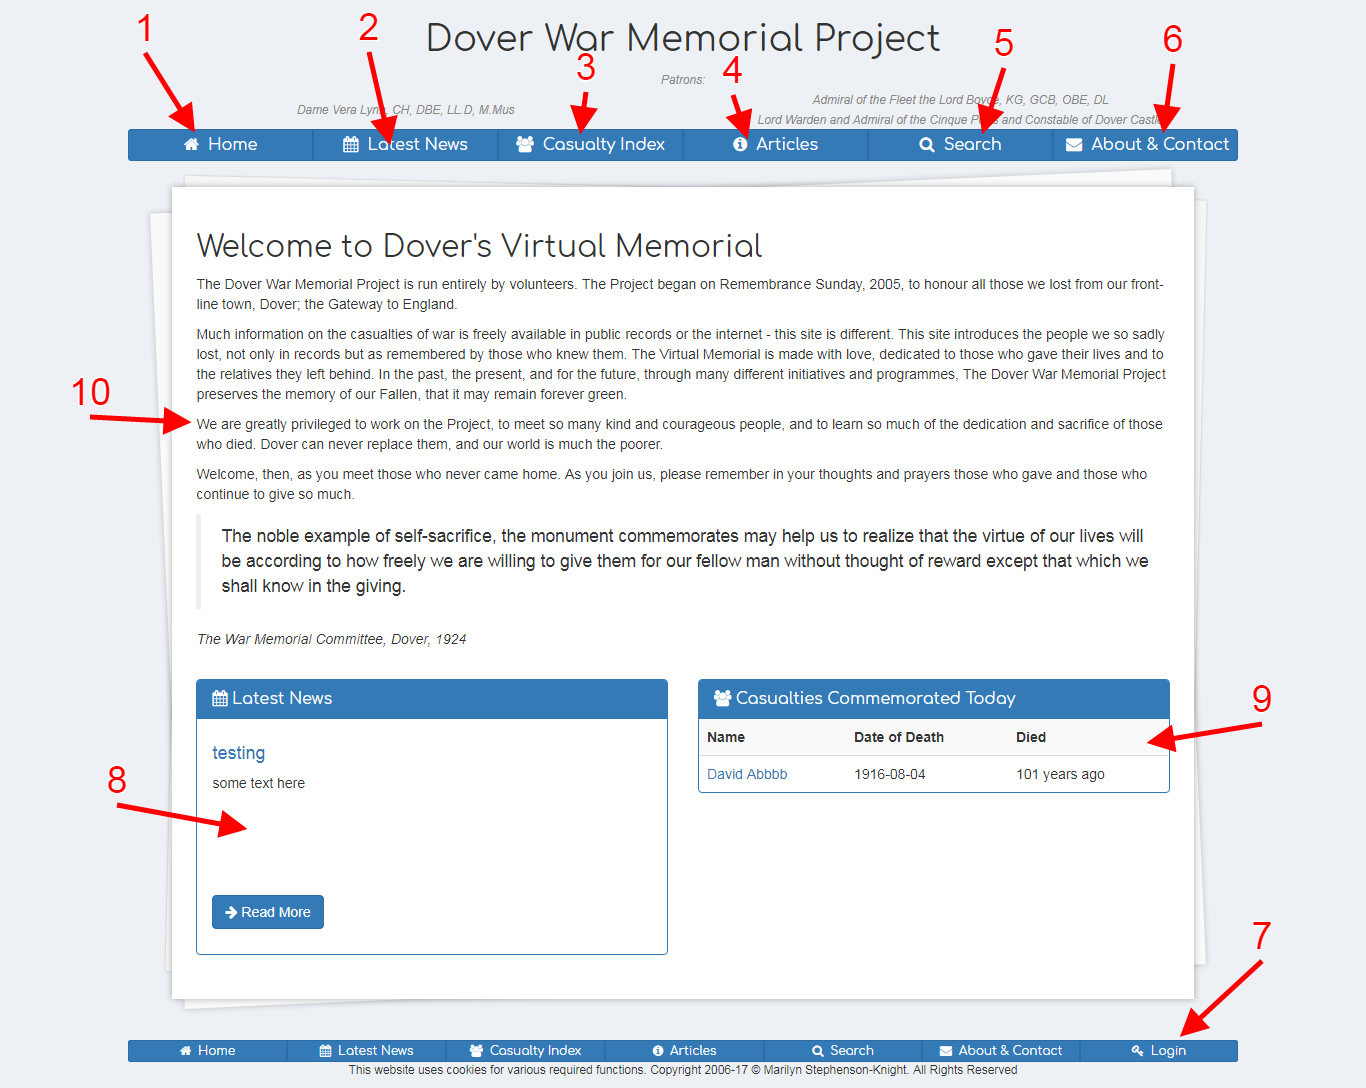
\includegraphics[width=.9\textwidth]{pics/home.png}
	\caption{Home Page}\label{fig:home}
\end{figure}

\newpage
\FloatBarrier
\subsection{How do I login?}\label{ssec:login}
To login, click the \textit{Login} button on the bottom menu bar (see \marker{7}\ on Figure~\ref{fig:home}). The login page is then loaded (Figure~\ref{fig:login}), which allows the user to login to the site to make various changes. \marker{1}\ is where the username must be entered with \marker{2}\ being the password field. \marker{3}\ submits this information.

\begin{warningBox}
There is no way of resetting your username or password, so ensure that you remember it
\end{warningBox}

\begin{figure}[h]
  \centering
 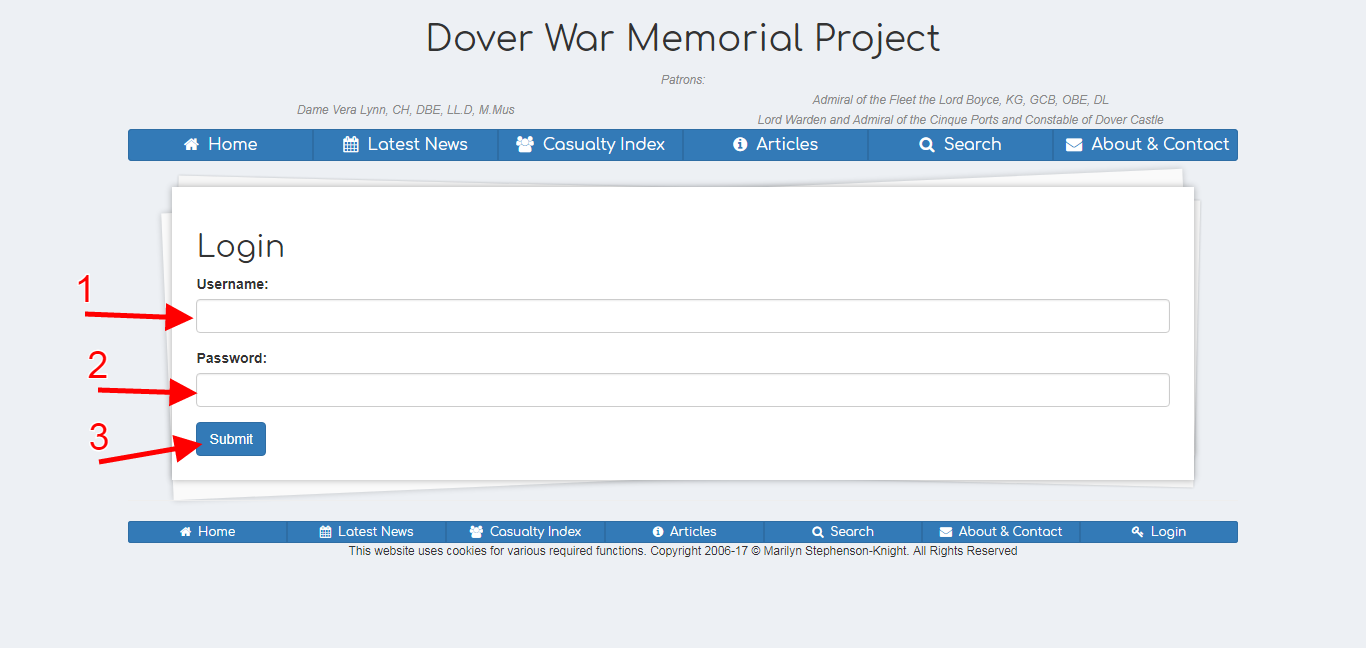
\includegraphics[width=.9\textwidth]{pics/login.png}
	\caption{Login Page}\label{fig:login}
\end{figure}

\newpage
\FloatBarrier
\subsection{How does the Home Page look after Login?}
Once a user has logged in, menu bars change. The top menu bar gains another row, with the login button on the bottom bar being replaced with a logout button, as can be seen in Figure~\ref{fig:home_login}. \marker{1}\ shows the currently logged in user, \marker{2}\ navigates to the config page (Section~\ref{sec:config}) and \marker{3}\ the admin help page (where this document is stored). \marker{4}\ and \marker{5}\ allow the user to logout. \marker{6} allows the user to edit the narrative text. These appear in numerous places across the site.

\begin{figure}[h]
  \centering
 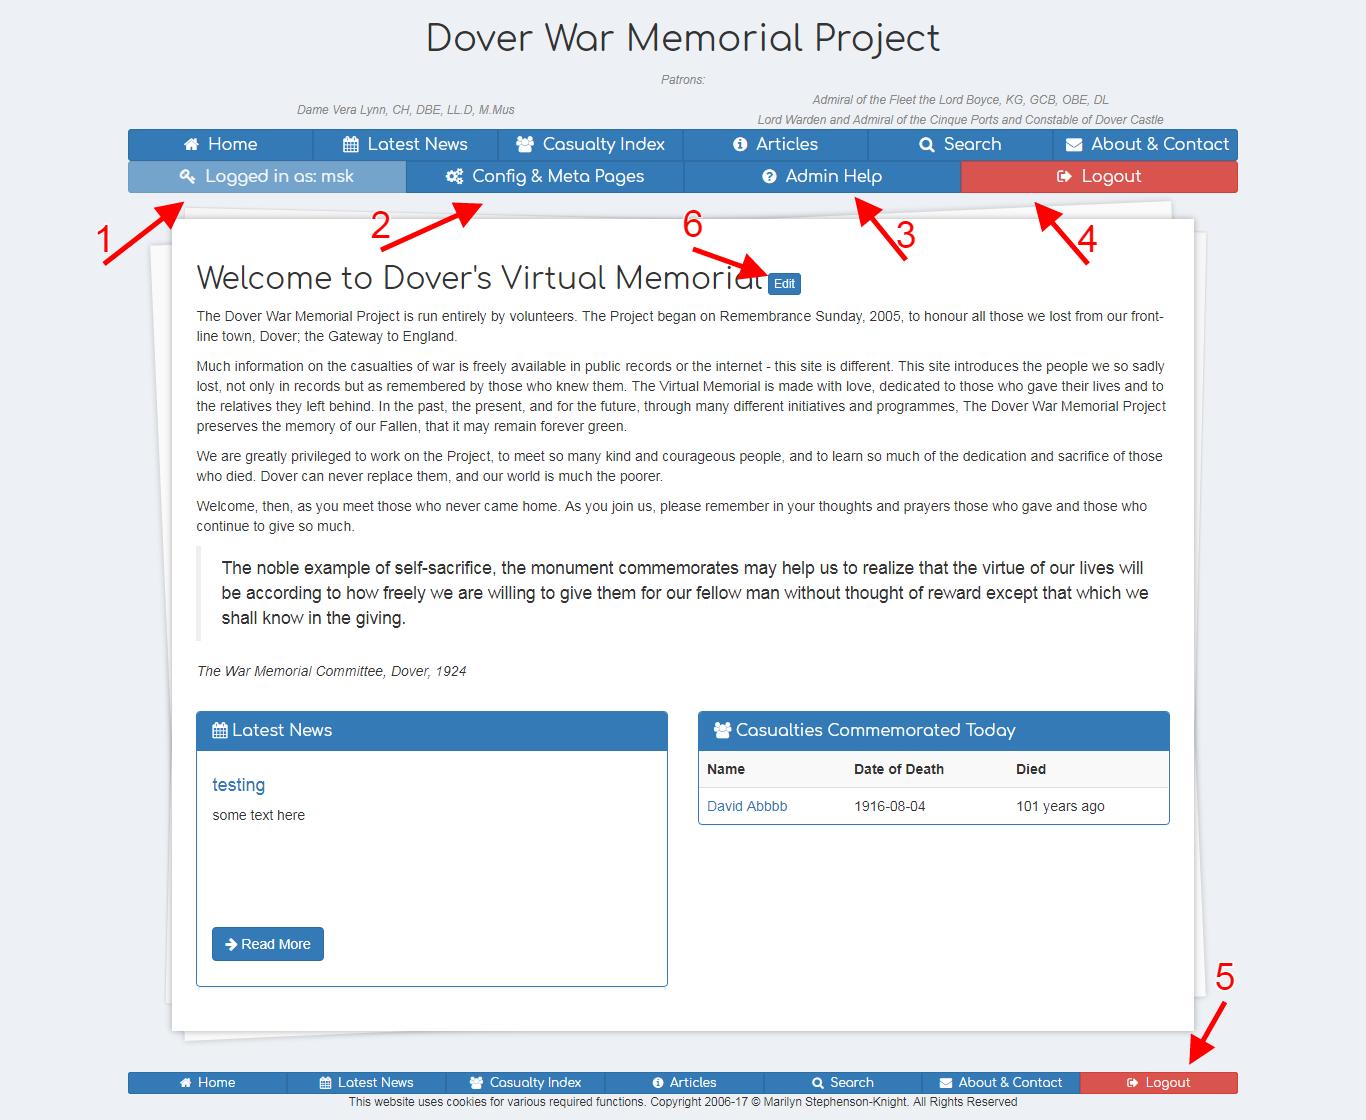
\includegraphics[width=.9\textwidth]{pics/home_login.png}
	\caption{Home Page after Login}\label{fig:home_login}
\end{figure}

\newpage
\FloatBarrier
\section{Site Updates}\label{sec:siteUpdate}
This section of the site contains two areas: Latest News, and a Change Log. The latest news section is for interesting updates and events that you may wish to bring attention to, in a similar way to the current latest news page. The most recent news article is also displayed on the home page.

The Change Log is a list of all the changes on the site (or rather, all the changes when you have entered a description of the change). This allows those visitors who wish to know what exactly is changing and when the ability to do so. It's also quite useful to show that the site is ``fresh'' and being regularly updates.

\subsection{How do I view a List of Updates?}\label{ssec:view_updates}

Navigate to Site Update section, by clicking the \textit{Latest News} link in either menu bar. A list of this year's updates will show, in a similar fashion to Figure~\ref{fig:view_updates}.

\begin{figure}[h]
  \centering
 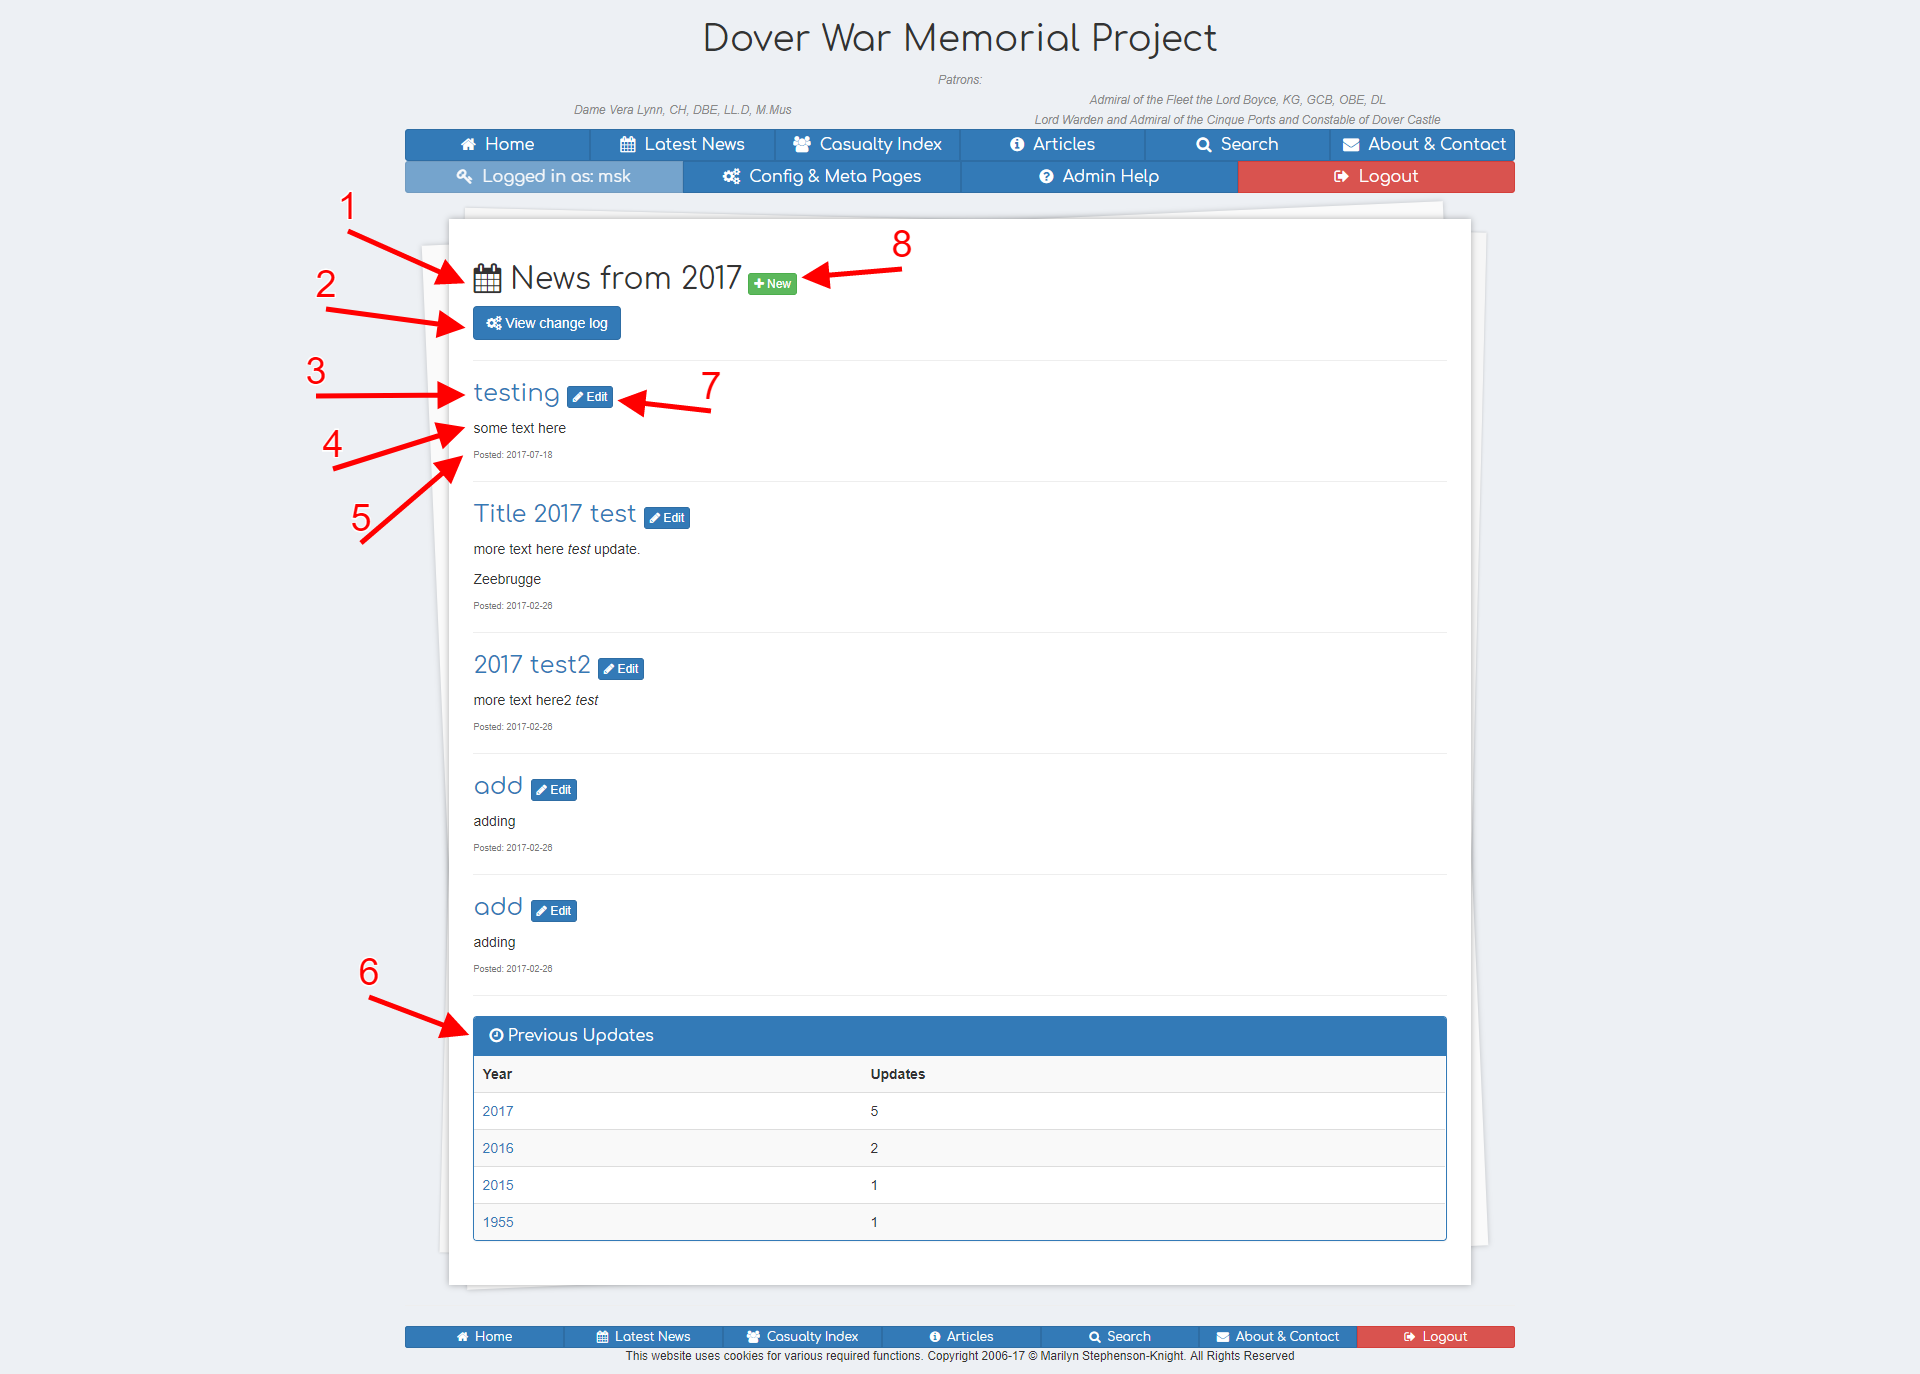
\includegraphics[width=.9\textwidth]{pics/view_updates.png}
	\caption{List of Site Updates}\label{fig:view_updates}
\end{figure}

\marker{1}\ indicates which year's updates are being shown, with \marker{2}\ providing a link to the change log, described in Section~\ref{ssec:changeLog}. Each update is displayed below that, with \marker{3}\ showing the title (and allowing the user to view an individual update, as in Section~\ref{ssec:view_update}), \marker{4}\ the content of that update and \marker{5}\ the date the site update was posted. \marker{6}\ shows a list of previous years and the number of site updates from those years. Clicking on a year will load the updates from the respective year. \marker{7}\ and \marker{8}\ allow the creation and editing of a site update, which is described in Section~\ref{ssec:edit_update}.

\newpage
\FloatBarrier
\subsection{How do I view a particular Update?}\label{ssec:view_update}
To view a particular update, click on the title of any update on the list of updates (\marker{3}\ in Figure~\ref{fig:view_updates}). A page will load similar to Figure~\ref{fig:view_update}. \marker{1}\ shows the title, \marker{2}\ the content of the update and \marker{3}\ the date the site update was posted. \marker{4}\ allows the user to return to the list of site updates for that year, while \marker{5} allows the user to edit this update, as described in Section~\ref{ssec:edit_update}.

\begin{figure}[h]
  \centering
 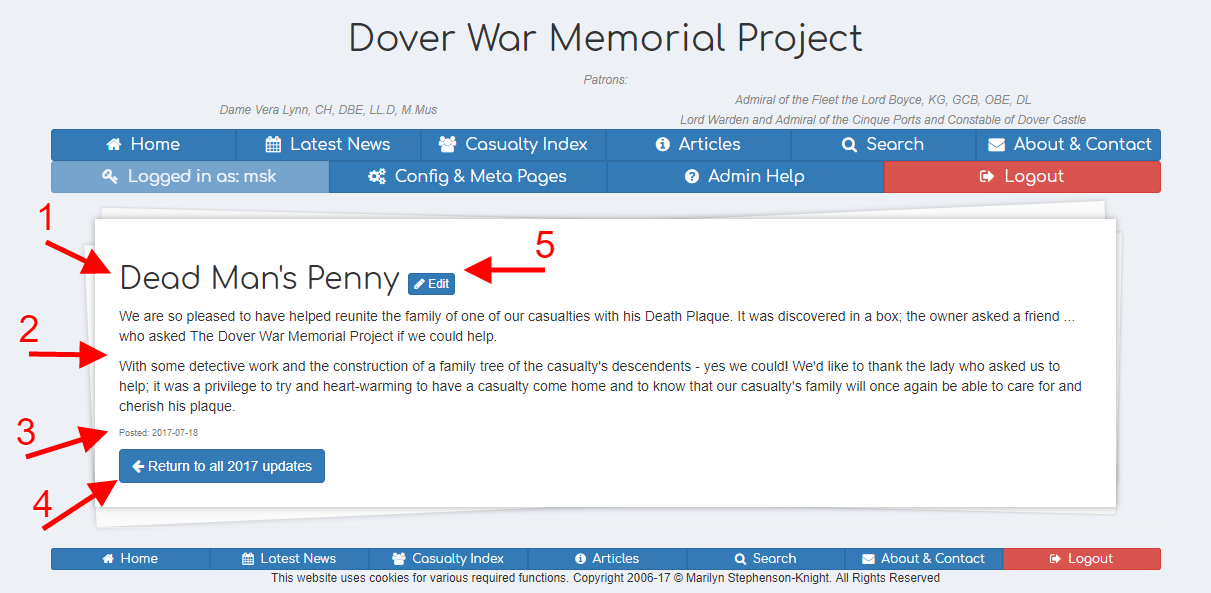
\includegraphics[width=.9\textwidth]{pics/view_update.png}
	\caption{Example of a Site Update}\label{fig:view_update}
\end{figure}

\newpage
\FloatBarrier
\subsection{How do I Add or Edit an Update?}\label{ssec:edit_update}
To create a new site update, use the \textit{Add} button on the list of updates (\marker{8}\ of Figure~\ref{fig:view_updates}. To edit an update, click the \textit{Edit} button next to the title of the update, either on the list of updates (\marker{7}\ on Figure~\ref{fig:view_updates}) or the page of a particular update (\marker{5}\ on Figure~\ref{fig:view_update}). Both methods will load a similar page, with the difference being that an Edit page will have boxes filled with data, as can be seen in Figure~\ref{fig:edit_update}.

\begin{figure}[h]
  \centering
 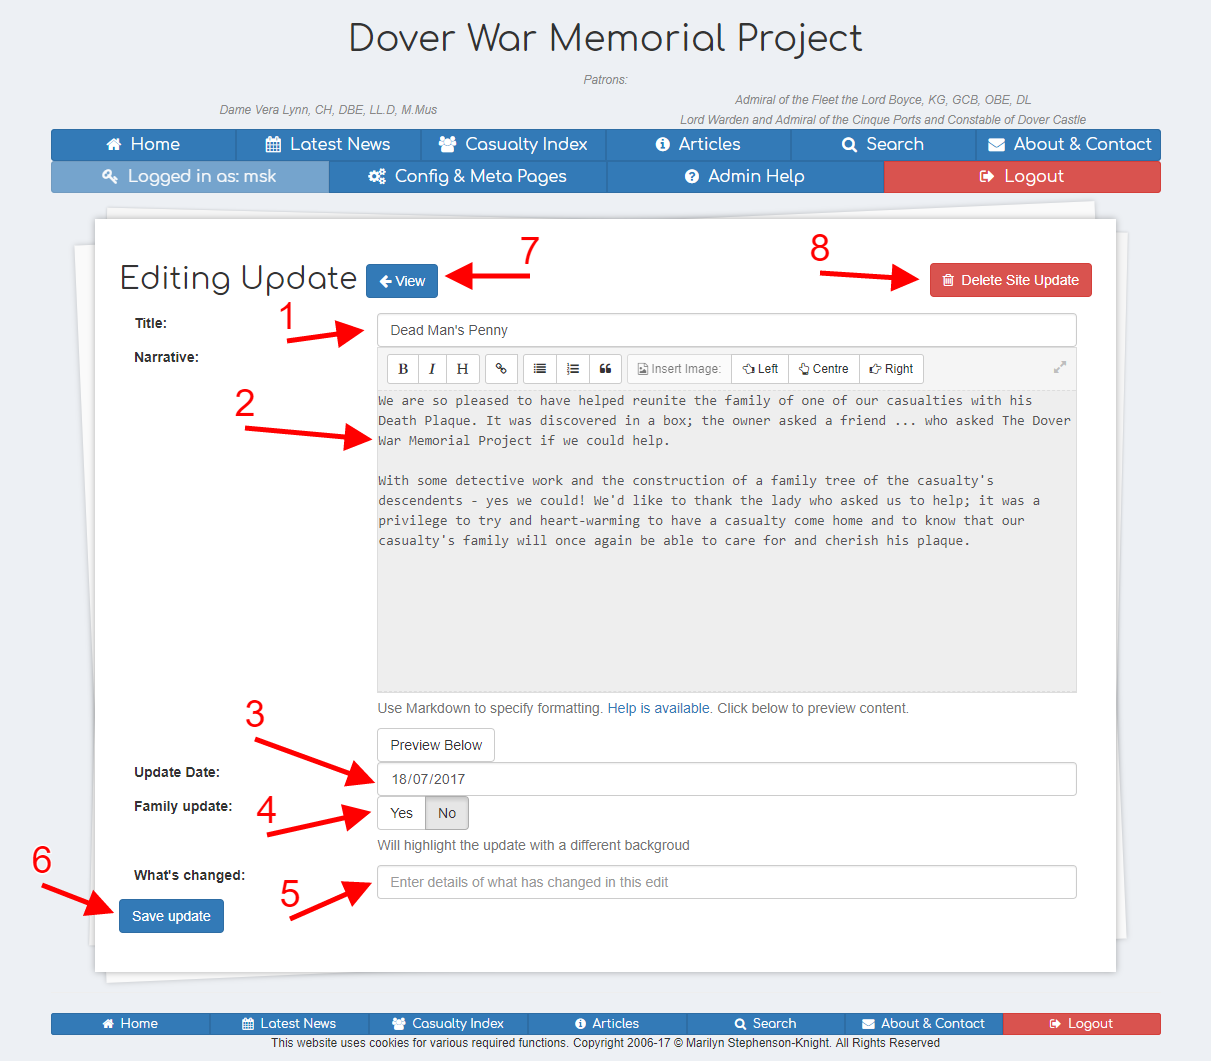
\includegraphics[width=.9\textwidth]{pics/edit_update.png}
	\caption{Example of Editing a Site Update}\label{fig:edit_update}
\end{figure}

\marker{1}\ allows the editing of the title of the site update, while \marker{2}\ allows the editing of the main content of the update. An explanation of the buttons around this area is described in Section~\ref{ssec:narrative}. \marker{3}\ shows the date this update was posted on. It is possible to set this in the future - if this is done, the update will not appear in list of updates until this date (for example, you could create a Christmas message that appears on the 25th December, without needing to log on then). A list of future updates is described in Section~\ref{ssec:config}.

\begin{infoBox}
The \texttt{title}, \texttt{content} and \texttt{date posted} fields must all be complete before the site update can be saved
\end{infoBox}

\marker{4}\ will show a slightly different background is this is a ``family update'' in a similar manner to the existing site. \marker{5}\ allows this edit to be recorded in the Change Log, if completed. Creating a new update, or substantially editing one, may be of interest so this field can be completed. For fixing a small typo, it is probably not worth it. \marker{6}\ saves this update, while \marker{7}\ returns to view this update, discarding any changes. \marker{8}\ allows the deletion of an update and is described in Section~\ref{ssec:delete_update}. The \textit{View} and \textit{Delete} buttons are not shown if this is a new memorial.

\FloatBarrier
\subsection{How do I delete an Update?}\label{ssec:delete_update}
To delete an update, navigate to its edit page, as described in Section~\ref{ssec:edit_update}. Using the \textit{Delete Site Update} button (\marker{8}\ in Figure~\ref{fig:edit_update}), will display a warning message similar to Figure~\ref{fig:delete_update}. Clicking on \textit{Cancel} (\marker{1}) will ignore this message, while \marker{2}\ will delete the site update.

\begin{warningBox}
Deletions cannot be undone
\end{warningBox}

\begin{figure}[h]
  \centering
 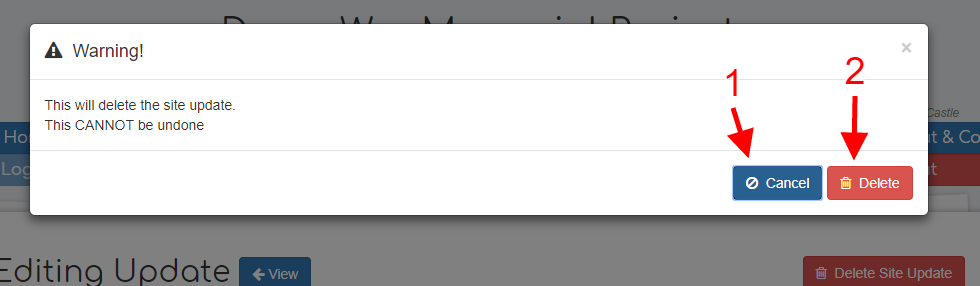
\includegraphics[width=.9\textwidth]{pics/delete_update.png}
	\caption{Deleting a Site Update}\label{fig:delete_update}
\end{figure}

\newpage
\FloatBarrier
\subsection{How do I view a List of Changes?}\label{ssec:changeLog}
To view the change log, navigate to the list of site updates (see Section~\ref{ssec:view_updates}) and click on the \textit{View change log} button, as shown by \marker{2}\ in Figure~\ref{fig:view_updates}. A page should load similar to Figure~\ref{fig:view_changes}.

\begin{figure}[h]
  \centering
 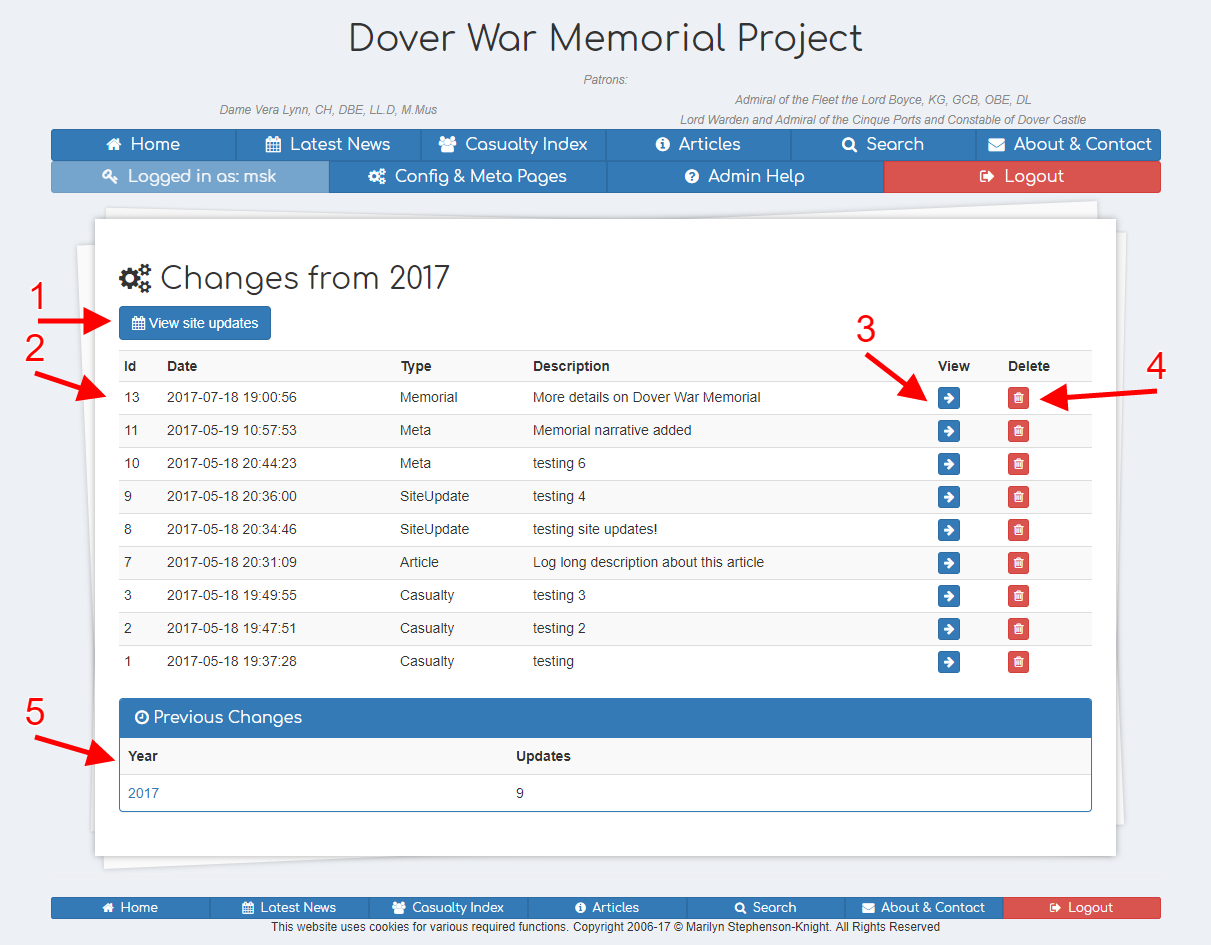
\includegraphics[width=.9\textwidth]{pics/view_changes.png}
	\caption{View the Change Log}\label{fig:view_changes}
\end{figure}

\marker{1}\ allows the user to return to the list of site updates (see Section~\ref{ssec:view_updates}). The table shown by \marker{2}\ lists the date of the change, the type of change, and the description entered. \marker{3} allows the quick navigation to the item changed, while \marker{4}\ allows the deletion of a change log item (see Section~\ref{ssec:delete_change}). \marker{5}\ indicates a summary of previous years' change log items, allowing a user to view a list of changes in the past.

\newpage
\FloatBarrier
\subsection{How do I delete an Change Log item?}\label{ssec:delete_change}
Navigate to the change log as described in Section~\ref{ssec:changeLog}. Next to the item in question, press the delete button (\marker{4} in Figure~\ref{fig:view_changes}). A panel should appear similar to Figure~\ref{fig:delete_change}. Clicking on \textit{Cancel} (\marker{1}) will ignore this message, while \marker{2}\ will delete the change log entry.

\begin{warningBox}
Deletions cannot be undone
\end{warningBox}

\begin{figure}[h]
  \centering
 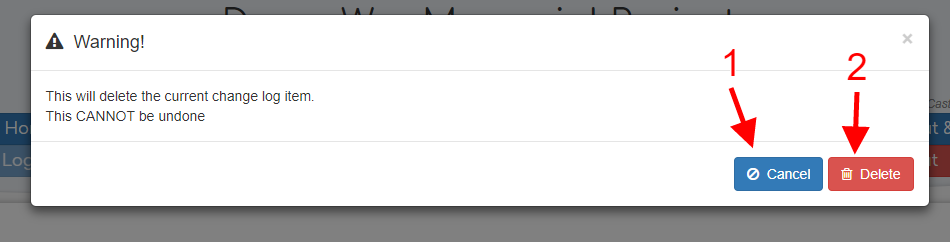
\includegraphics[width=.9\textwidth]{pics/delete_change.png}
	\caption{Deleting a Change Log Entry}\label{fig:delete_change}
\end{figure}

\newpage
\FloatBarrier
\section{Casualty Index}\label{sec:casualtyIndex}

The casualty index is the main section of the site, and therefore has a lot of details associated with it. Casualties are grouped into one or more memorials, with a few main ones shown in more prominence on the main memorial list (the same ones that are shown on the old site). Lists of casualties are displayed on each memorial's page. There is also a memorial map, which shows the various memorials on a interactive map. A casualty as the same narrative before, along with their pictures, as well as a section full of data - used to create the relational and searchable database.

\subsection{How do I view a List of all Memorials?}\label{ssec:view_memorials}
Navigate to the list of memorials by clicking the \textit{Casualty Index} button on the top or bottom menu bar. A page should load similar to Figure~\ref{fig:view_memorials}.

\begin{figure}[h]
  \centering
 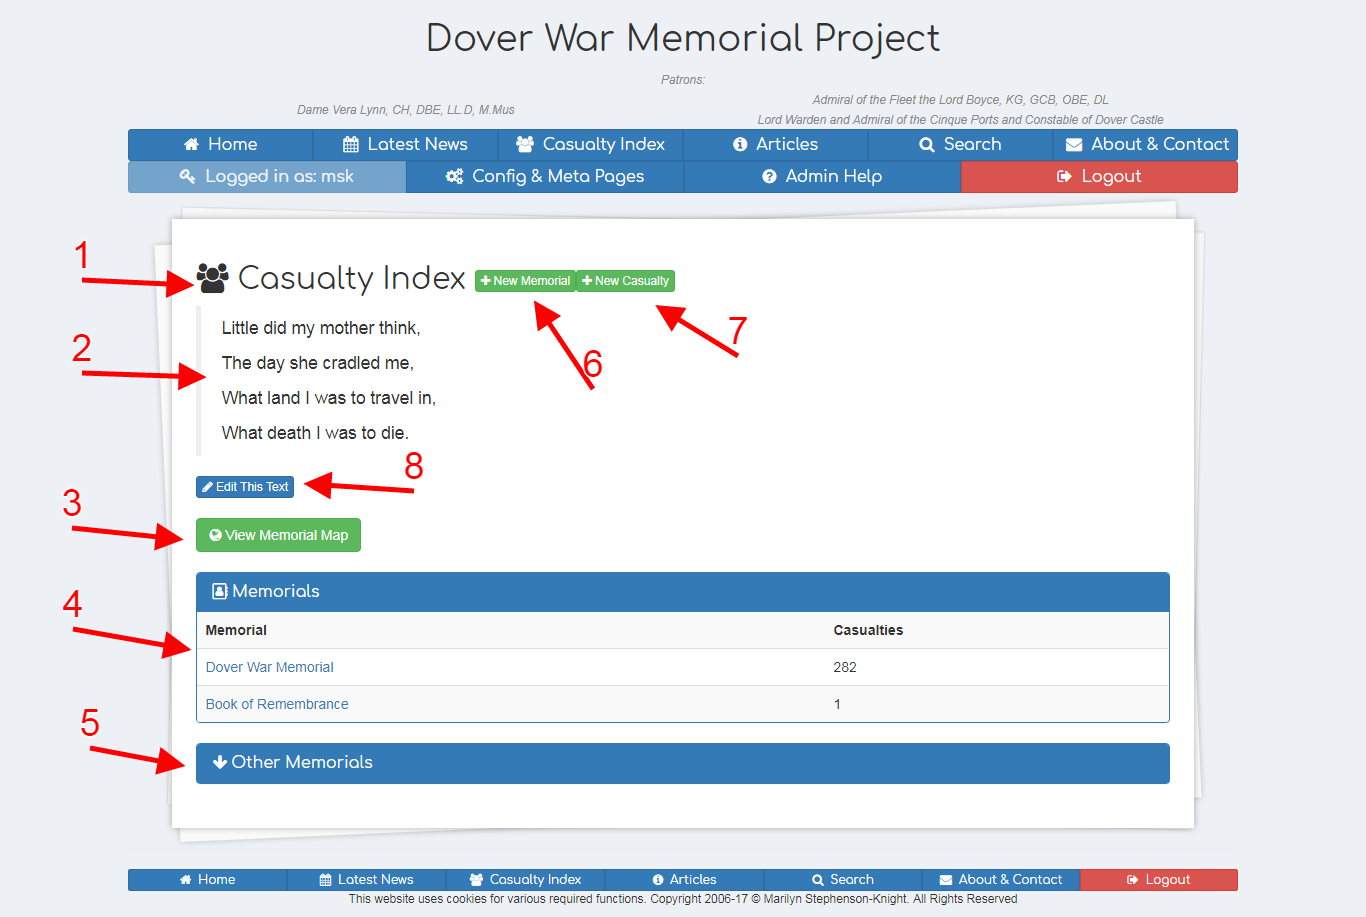
\includegraphics[width=.9\textwidth]{pics/view_memorials.png}
	\caption{View the List of Memorials}\label{fig:view_memorials}
\end{figure}

\marker{1}\ shows the title of the page, while \marker{2}\ provides some narrative content (which can be edited using \marker{8}). \marker{3}\ links to the memorial map, while the list of memorials are indicated by \marker{4}\. the name of the memorial and the number of casualties are shown. \marker{5}\ allows the user to also view the other memorials, which are displayed in the same way. \marker{6}\ and \marker{7}\ allow the creation of a new memorial and casualty respectively.

\newpage
\FloatBarrier
\subsection{How do I view the Memorial Map?}
To view the memorial map, navigate to the list of memorials (see Section~\ref{ssec:view_memorials}) and click on the \textit{Memorial Map} button, as shown by \marker{3}\ in Figure~\ref{fig:view_memorials}. A page should load similar to Figure~\ref{fig:view_map}.

\begin{figure}[h]
  \centering
 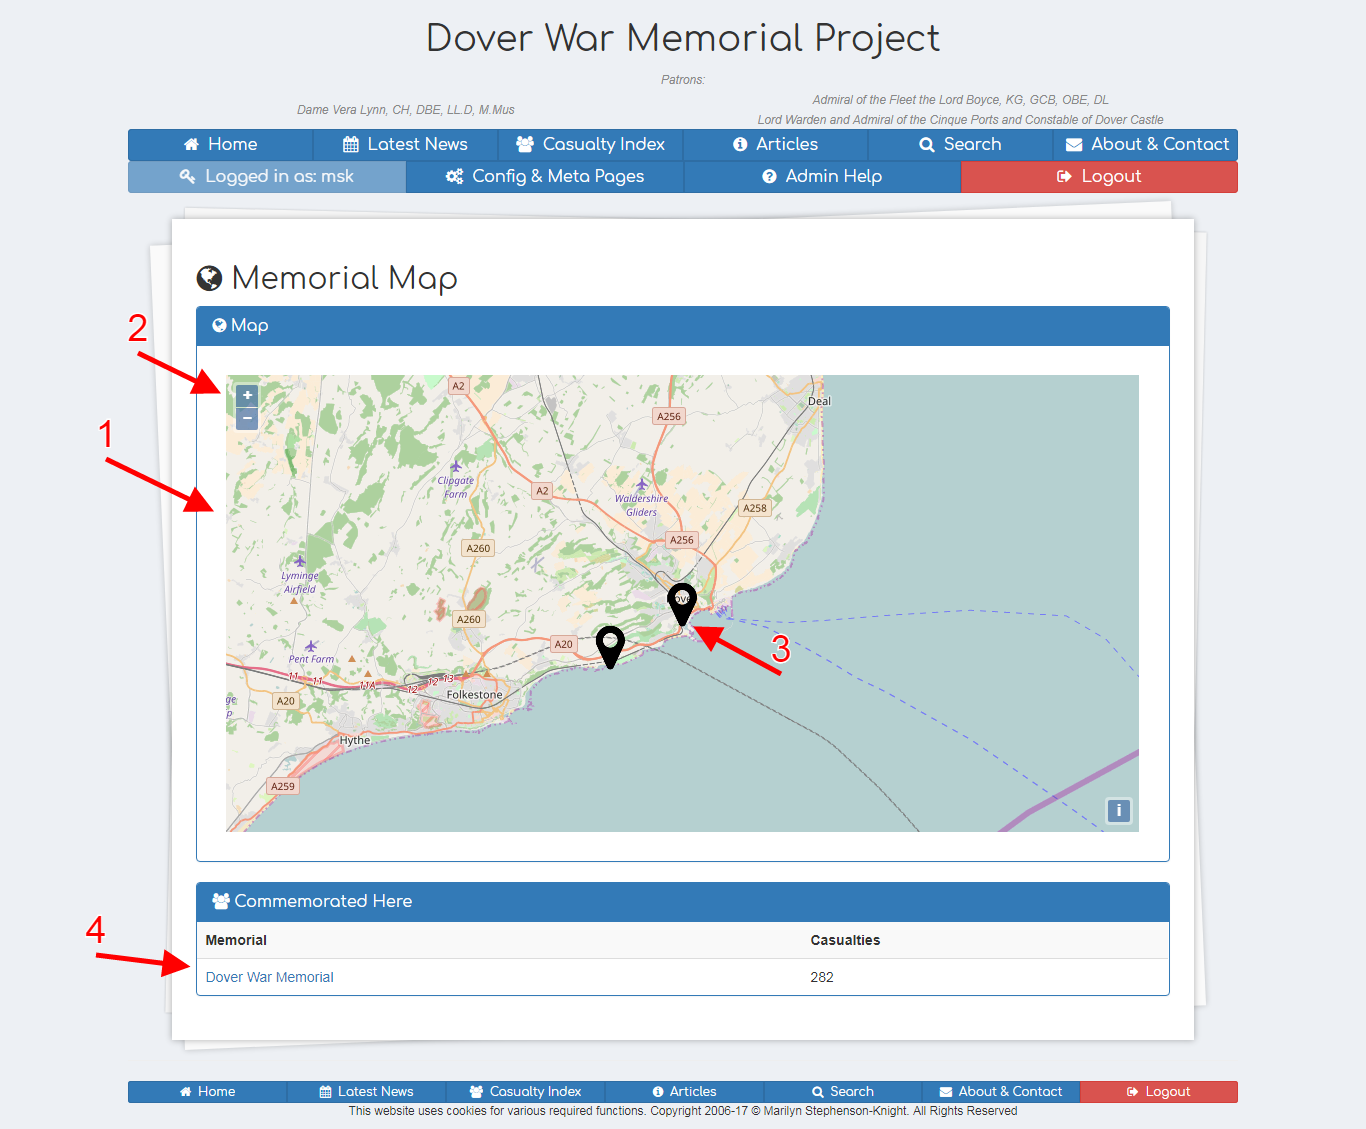
\includegraphics[width=.9\textwidth]{pics/view_map.png}
	\caption{View the Memorial Map}\label{fig:view_map}
\end{figure}

The main map window is shown in \marker{1}\ with some navigation buttons displayed in \marker{2}. The map uses standard navigation features: dragging, scrolling, etc. Clicking on a black pin, as indicated by \marker{3}, will show a panel below (\marker{4}) detailing the name and number of casualties at that memorial.
\begin{infoBox}
Only memorials with latitude and longitude information are displayed on this map, and by default, it will centre on Dover.
\end{infoBox}

\newpage
\FloatBarrier
\subsection{How do I view a particular Memorial?}
To view the memorial map, navigate to the list of memorials (see Section~\ref{ssec:view_memorials}) and click on the name of any memorial. A page will load similar to Figure~\ref{fig:view_memorial}.

\begin{figure}[h]
  \centering
 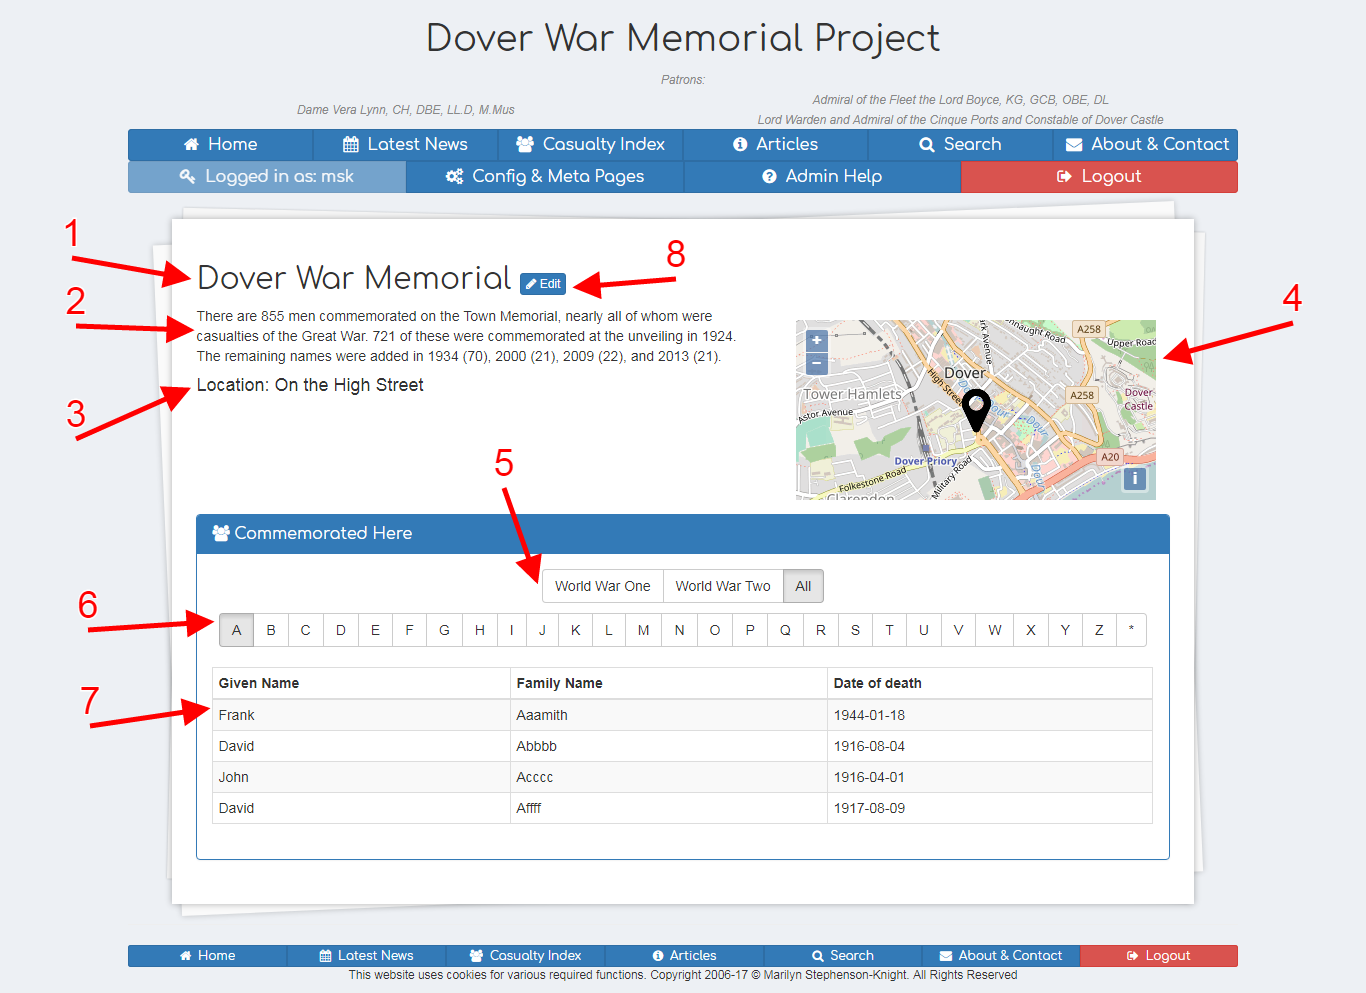
\includegraphics[width=.9\textwidth]{pics/view_memorial.png}
	\caption{View a particular memorial}\label{fig:view_memorial}
\end{figure}

\marker{1}\ gives the title of the memorial, while \marker{2}\ displays the narrative content, editable using the button indicated by \marker{8}. A text description of the location is shown by \marker{3}\ (for example, if the memorial is a book, or perhaps a grave reference number), with a map shown by \marker{4}. \marker{5}\ allows the user to filter casualties by the two World Wars, or by all wars, while \marker{6}\ allows the filtering by surname. The list of filtered casualties is indicated by \marker{7} and navigates to that casualty's particular page.

\begin{infoBox}
If no latitude or longitude has been set then the map is not displayed.
\end{infoBox}

\newpage
\FloatBarrier
\subsection{How do I Add or Edit a Memorial?}\label{ssec:edit_memorial}
To create a new memorial, use the \textit{New Memorial} button on the list of memorials (\marker{6}\ of Figure~\ref{fig:view_memorials}). To edit an update, click the \textit{Edit} button next to the title of the memorial on the page of a particular memorial (\marker{8}\ on Figure~\ref{fig:view_memorial}). Both methods will load a similar page, with the difference being that an Edit page will have boxes filled with data, as can be seen in Figure~\ref{fig:edit_memorial}.

\begin{figure}[h]
  \centering
 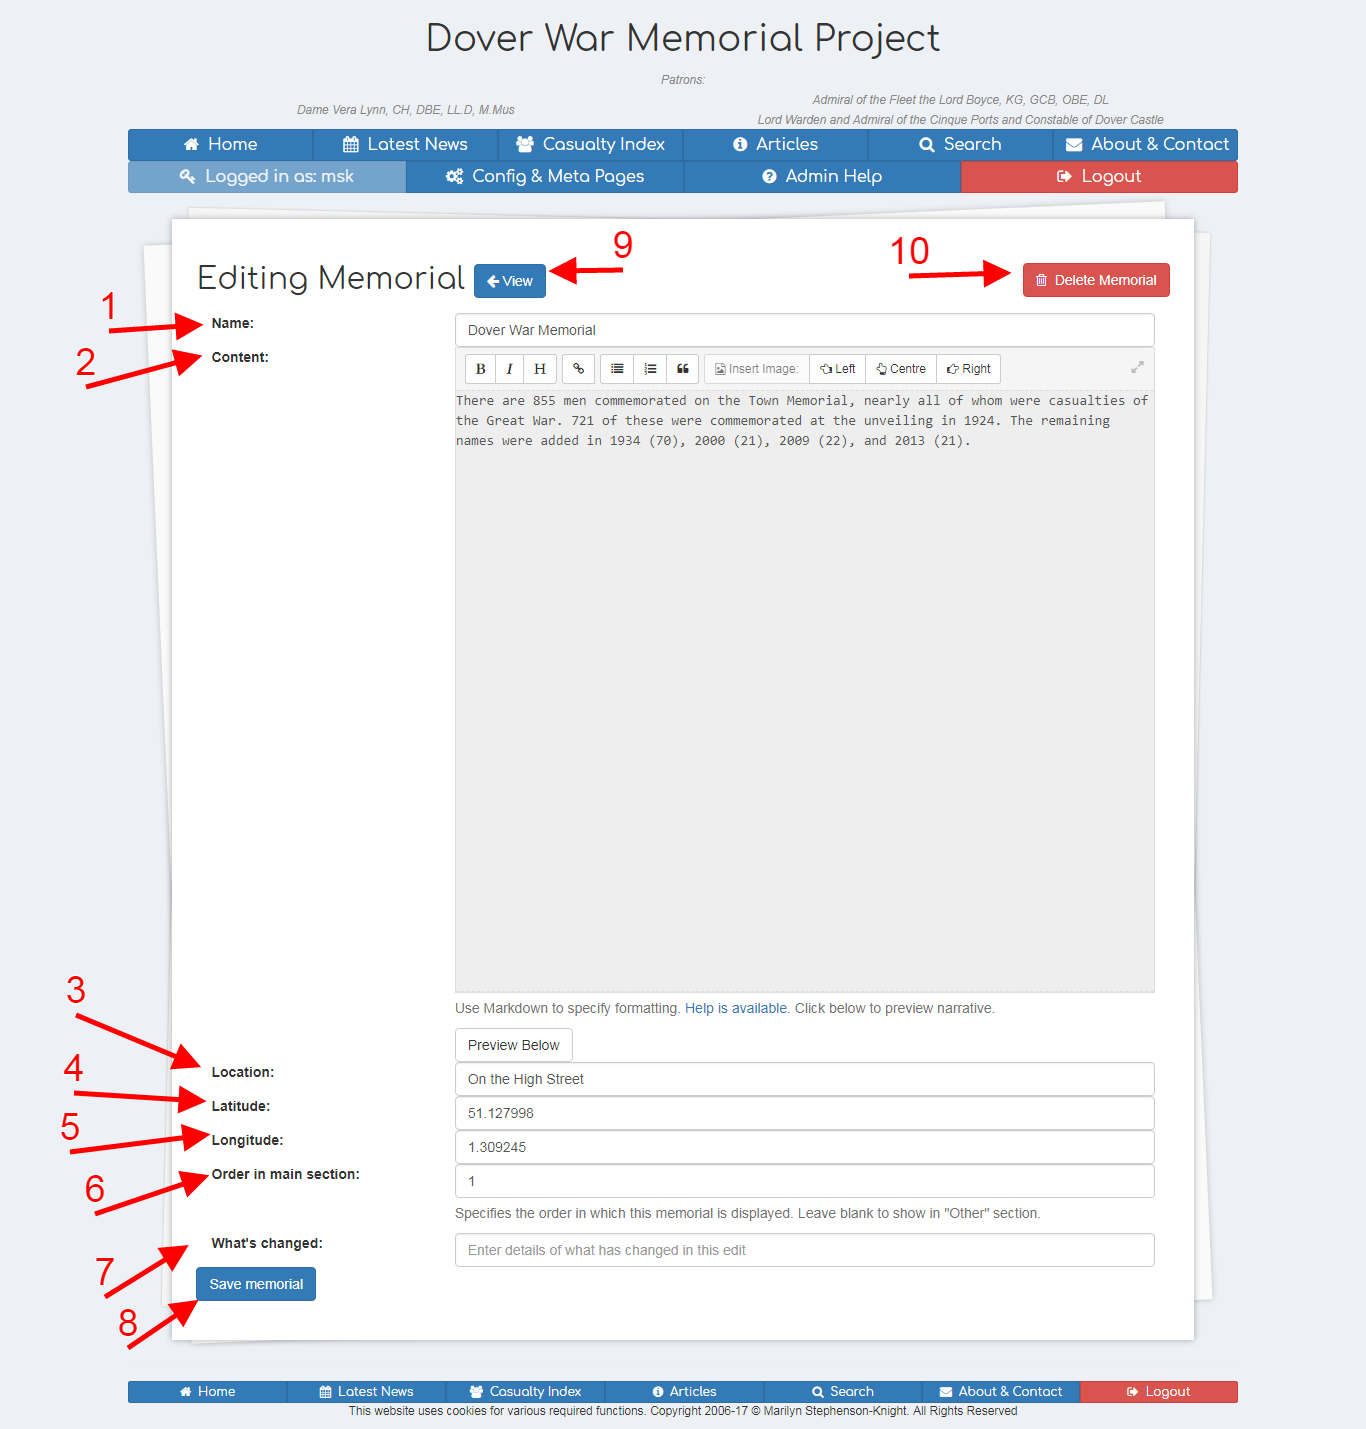
\includegraphics[width=.9\textwidth]{pics/edit_memorial.png}
	\caption{Editing a Memorial}\label{fig:edit_memorial}
\end{figure}

\marker{1}\ indicates the name of the memorial, with \marker{2}\ indicating the narrative content. An explanation of the buttons around this area is described in Section~\ref{ssec:narrative}. \marker{4}\ indicates the text description of the location of the memorial, while \marker{4}\ and \marker{5}\ contain the latitude and longitude (as decimal numbers). 

\begin{infoBox}
On Google Maps, right click and select \textit{What's here?}. At the bottom of the screen, the latitude and longitude of the clicked location is shown.
\end{infoBox}

\marker{6}\ indicates the order in which this memorial should appear in the main list of memorials. If this memorial should not appear in the main list, then leave this blank. The lower a number, the higher it will be displayed on the list. \marker{7}\ allows this edit to be recorded in the Change Log, if completed. Creating a new update, or substantially editing one, may be of interest so this field can be completed. For fixing a small typo, it is probably not worth it. \marker{8}\ saves this memorial, while \marker{9}\ returns to view this memorial, discarding any changes. \marker{10}\ allows the deletion of an update and is described in Section~\ref{ssec:delete_memorial}. The \textit{View} and \textit{Delete} buttons are not shown if this is a new memorial.

\begin{infoBox}
The \texttt{name} and \texttt{content} fields must all be complete before the site update can be saved
\end{infoBox}

\FloatBarrier
\subsection{How do I delete a Memorial?}\label{ssec:delete_memorial}
To delete a memorial, navigate to its edit page, as described in Section~\ref{ssec:edit_memorial}. Using the \textit{Delete Memorial} button (\marker{10}\ in Figure~\ref{fig:edit_memorial}), will display a warning message similar to Figure~\ref{fig:delete_memorial}. Clicking on \textit{Cancel} (\marker{1}) will ignore this message, while \marker{2}\ will delete the memorial.

\begin{warningBox}
Any casualties with this memorial will have it removed. This may mean some casualties have no memorial and therefore will be displayed in a list as described in Section~\ref{ssec:config}.\\
Deletions cannot be undone
\end{warningBox}

\begin{figure}[h]
  \centering
 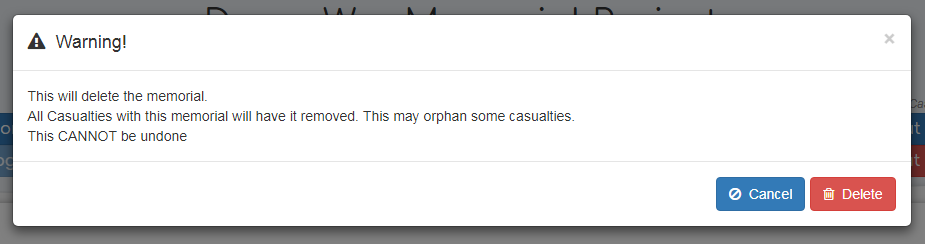
\includegraphics[width=.9\textwidth]{pics/delete_memorial.png}
	\caption{Deleting a Site Update}\label{fig:delete_memorial}
\end{figure}

\newpage
\FloatBarrier
\subsection{How do I view a Casualty?}\label{ssec:view_casualty}
To navigate to a particular casualty, navigate to a particular memorial and choose the casualty from the list (\marker{7}\ from Figure~\ref{fig:view_memorial}). It is also possible to arrive at a casualty from the home page if they are commemorated on this particular date. A page should load similar to Figure~\ref{fig:view_casualty}.

\begin{figure}[h]
  \centering
 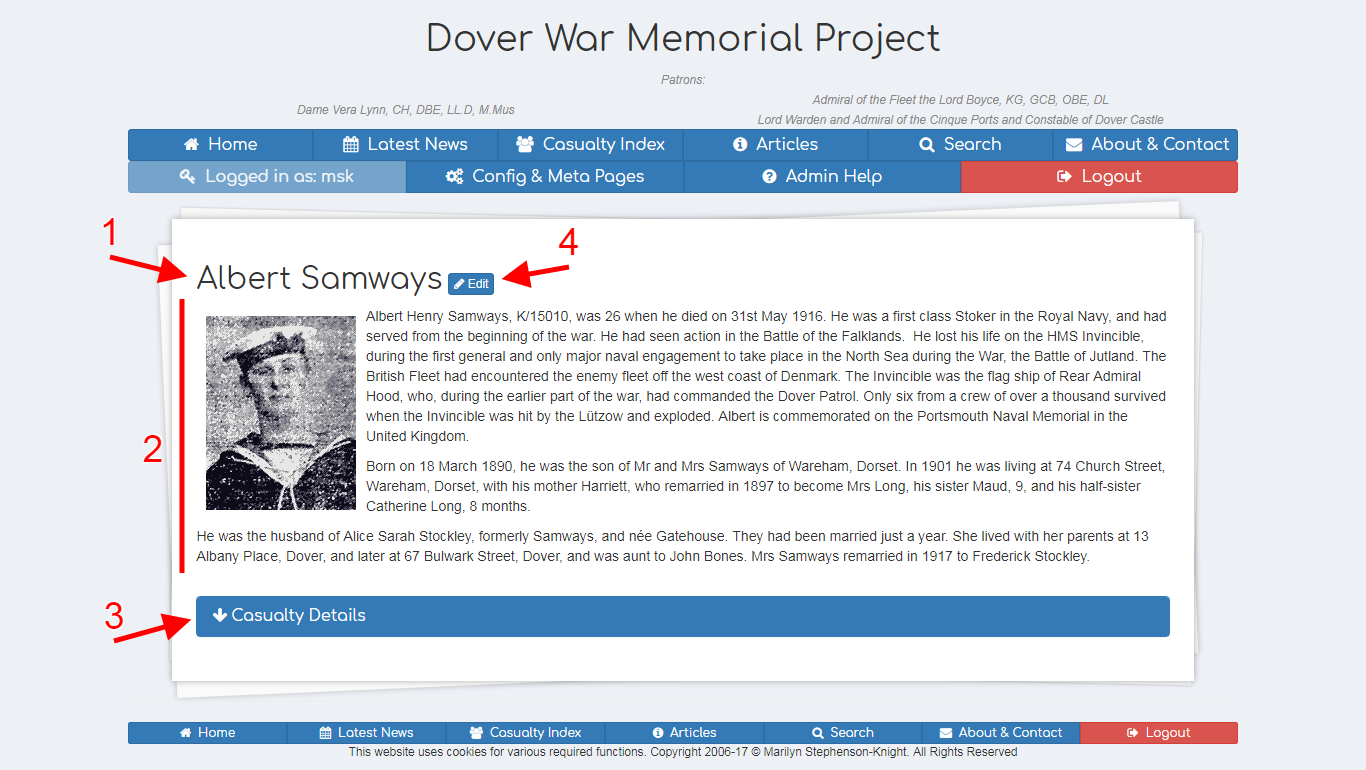
\includegraphics[width=.9\textwidth]{pics/view_casualty.png}
	\caption{Viewing a Casualty}\label{fig:view_casualty}
\end{figure}

\marker{1}\ indicates the name of this casualty (their given name and family name). \marker{2}\ indicates the main narrative section of the casualty, including any pictures. \marker{3}\ shows the data for the particular casualty, while \marker{4} indicates a button that allows the editing of this casualty (see Section~\ref{ssec:edit_casualty}).

\newpage
\FloatBarrier
\subsection{How do I view a Casualty's Data?}\label{ssec:view_casualty_data}
Clicking on \marker{3}\ on Figure~\ref{fig:view_casualty} will adjust the page to show the full data of this casualty, as shown in Figure~\ref{fig:view_casualty_data}.

\begin{figure}[h]
  \centering
 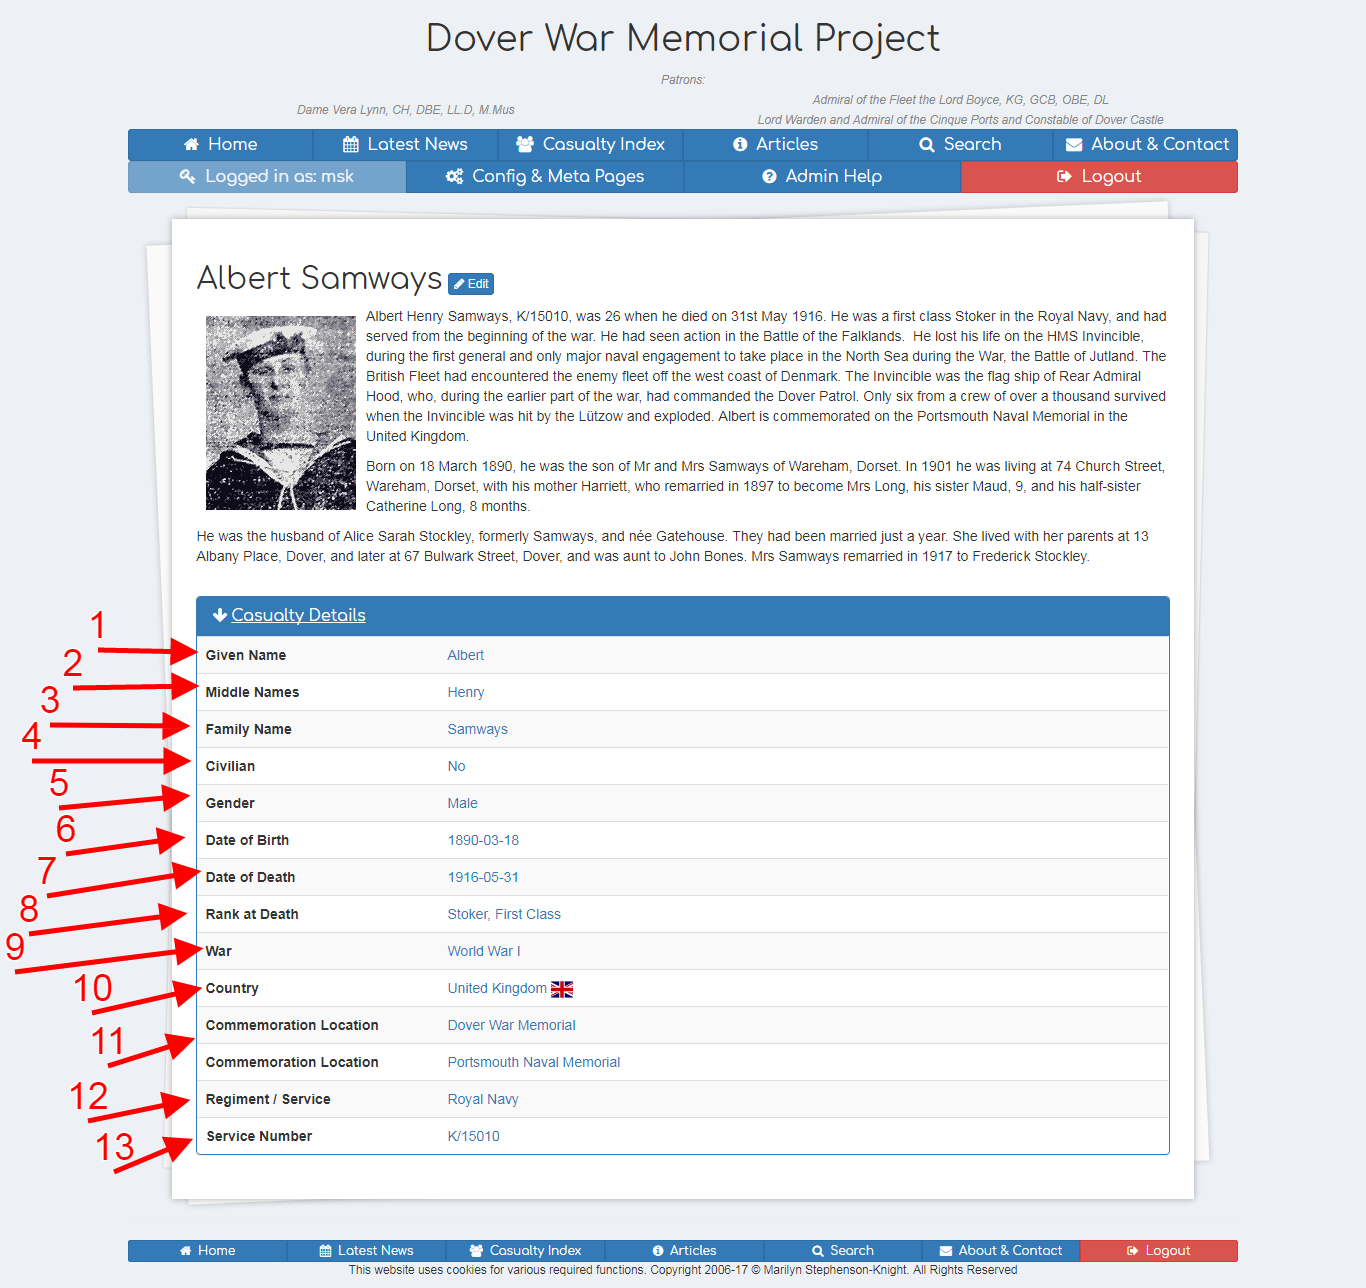
\includegraphics[width=.9\textwidth]{pics/view_casualty_data.png}
	\caption{Viewing a Casualty}\label{fig:view_casualty_data}
\end{figure}

\marker{1}, \marker{2}\ and \marker{3}\ all indicate the full name of the given casualty, while \marker{4}\ indicates if they are a civilian. \marker{5}\ indicates their gender and \marker{6}\ and \marker{7}\ indicate the casualty's date of birth and death respectively. \marker{8}\ indicates their rank at death, while \marker{9}\ indicates the particular war they died in. \marker{10}\ indicates the country for which they served, while \marker{11}\ shows any commemoration locations (in this example, there are two). \marker{12}\ indicates the Regiment or Service, while \marker{13}\ indicates any service numbers the casualty may have had. Any relations would be displayed below, although this casualty has none.

\begin{infoBox}
If a particular piece of data is not available, then the row will be missing.\\
Clicking on a piece of data will create a search based around it.
\end{infoBox}

\newpage
\FloatBarrier
\subsection{How do I Add or Edit a Casualty?}\label{ssec:edit_casualty}
To create a new casualty, use the \textit{Add} button on the list of memorials (\marker{7}\ of Figure~\ref{fig:view_memorials}. To edit a a casualty, click the \textit{Edit} button next to the title of the update on the page of a particular casualty (\marker{4}\ on Figure~\ref{fig:view_casualty}). Both methods will load a similar page, with the differences being that an Edit page will have boxes filled with data and will not have a \textit{View} or \textit{Delete} button, as can be seen in Figures~\ref{fig:edit_casualty} and ~\ref{fig:edit_casualty2}.
\begin{infoBox}
The Add page will also only display the first section until the casualty is saved.
\end{infoBox}

\begin{figure}[h]
  \centering
 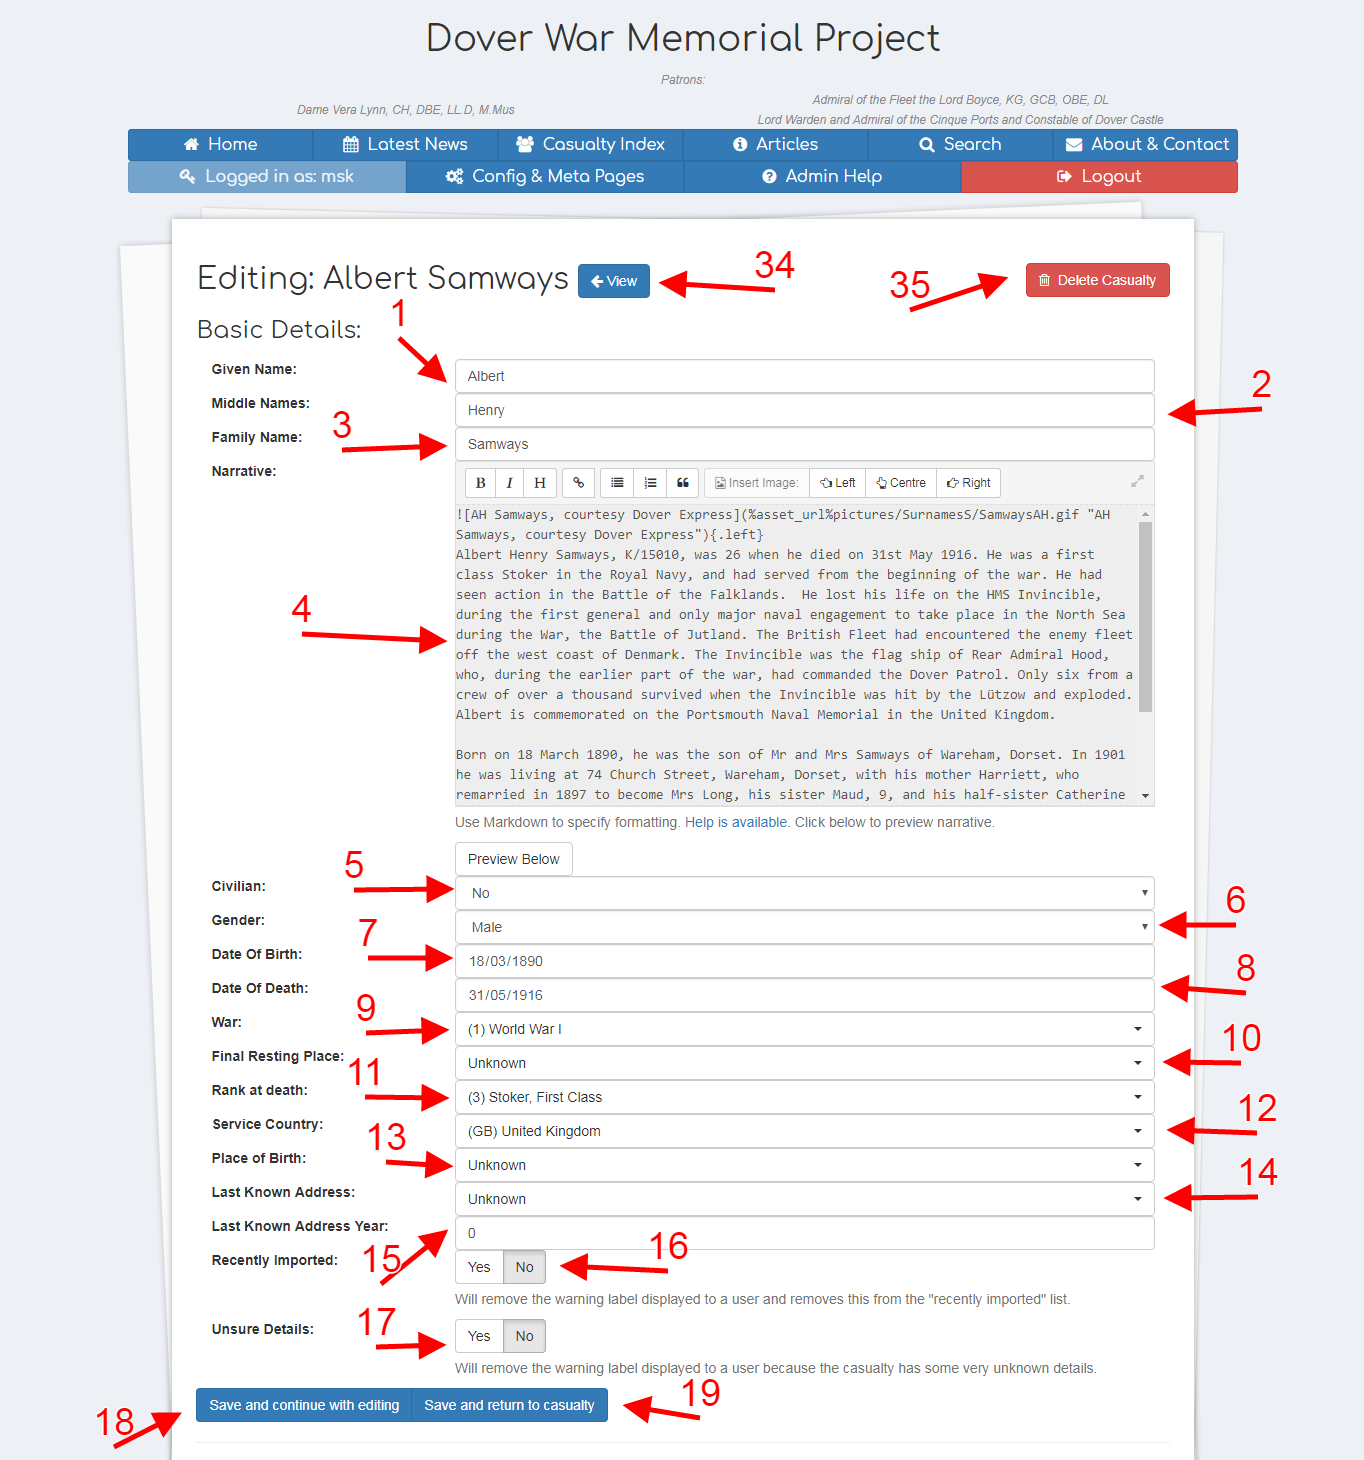
\includegraphics[width=.9\textwidth]{pics/edit_casualty.png}
	\caption{Example of Editing a Casualty (1)}\label{fig:edit_casualty}
\end{figure}

\begin{figure}[h]
  \centering
 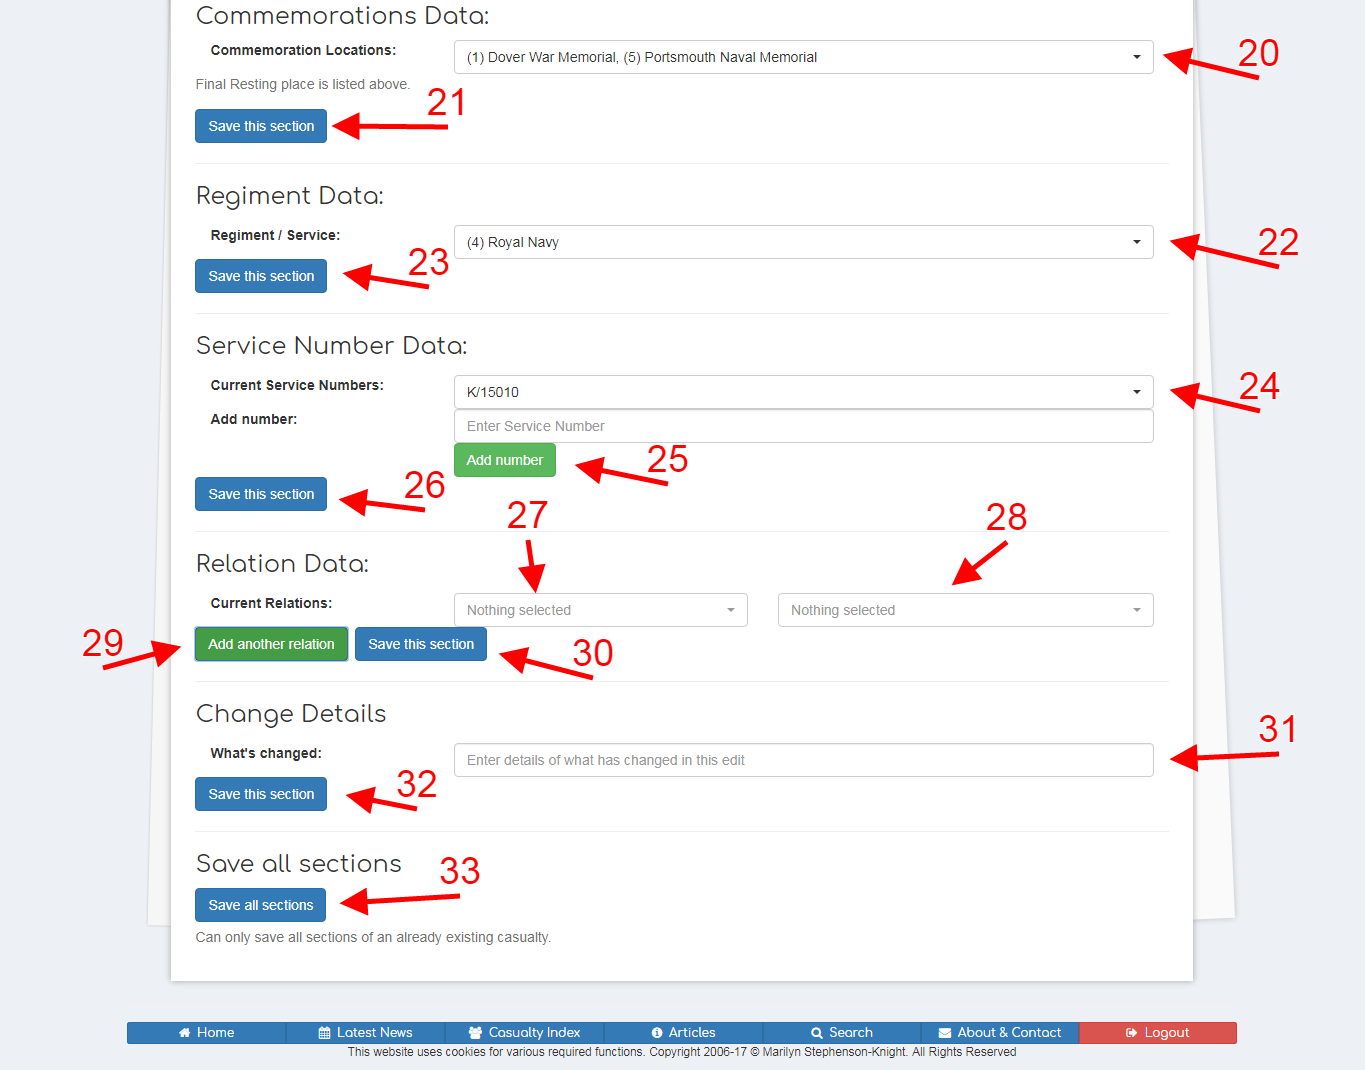
\includegraphics[width=.9\textwidth]{pics/edit_casualty2.png}
	\caption{Example of Editing a Casualty (2)}\label{fig:edit_casualty2}
\end{figure}

\marker{1}, \marker{2}\ and \marker{3}\ all indicate the full name of the given casualty, while \marker{4}\ contains the narrative content for this casualty. An explanation of the buttons around this area is described in Section~\ref{ssec:narrative}. \marker{5}\ identifies a dropdown box that allows the selection of the casualty's civilian status, while \marker{6} determines their gender. \marker{7}\ and \marker{8}\ indicate the casualty's date of birth and death. When hovering over these fields, a dropdown is possible that displays a calendar - this may not be too useful for the dates that are likely to be in these fields, however. Next, \marker{9}\ provides a dropdown with a list of potential wars this casualty may have died in, while \marker{10}\ allows the selection of their final resting place. \marker{12}\ provides another dropdown, this time for the service country, with \marker{13}\ allows for the selection of the casualty's place of birth. \marker{14}\ and \marker{15}\ allow for the selection of the Last Known Address and the year that it was known. \marker{16}\ indicates if this casualty was recently imported - if so, a message is displayed to the user informing that the data may not be complete. \marker{17}\ indicates if some details are unknown, and if so, a message is displayed to the user. This replaces the previous method of placing an asterisk next to a casualty's name.

\begin{infoBox}
Many dropdowns allow searching. Type to limit the results shown. \\
The \texttt{name} and \texttt{content} fields must all be complete before the site update can be saved.
\end{infoBox}

\newpage
\FloatBarrier
\subsection{How do I delete a Casualty?}\label{ssec:delete_casualty}


\section{Articles}\label{sec:articles}
articles
\subsection{How do I view the list of Articles?}
\subsection{How do I view a particular Article?}
\subsection{How do I Add or Edit an Article?}
\subsection{How do I delete an Article?}

\section{Search}\label{sec:search}
Search
\subsection{How do I perform a Text Search?}
\subsection{How do I perform a Data Search?}
\subsection{How do I view the Search Results?}

\section{Config \& Meta Pages}\label{sec:config}
Config
\subsection{How do I view the config page?}\label{ssec:config}
\subsection{How do I view a list of Places?}
\subsection{How do I Add, Edit or Delete a Place?}
\subsection{How do I view a list of Ranks?}
\subsection{How do I Add, Edit or Delete a Rank?}
\subsection{How do I view a list of Regiment / Service?}
\subsection{How do I Add, Edit or Delete a Regiment / Service?}
\subsection{How do I view a list of Relation Types?}
\subsection{How do I Add, Edit or Delete a Relation Type?}
\subsection{How do I view a list of Service Country?}
\subsection{How do I Add, Edit or Delete a Service Country?}
\subsection{How do I view a list of Wars?}
\subsection{How do I Add, Edit or Delete a War?}
\subsection{How do I view a List of Recently Uploaded Casualties?}

\section{Others}
Others
\subsection{How do I use the Narrative Buttons?}\label{ssec:narrative}

\end{document}